
% Default to the notebook output style

    


% Inherit from the specified cell style.




    
\documentclass[11pt]{article}

    
    
    \usepackage[T1]{fontenc}
    % Nicer default font (+ math font) than Computer Modern for most use cases
    \usepackage{mathpazo}

    % Basic figure setup, for now with no caption control since it's done
    % automatically by Pandoc (which extracts ![](path) syntax from Markdown).
    \usepackage{graphicx}
    % We will generate all images so they have a width \maxwidth. This means
    % that they will get their normal width if they fit onto the page, but
    % are scaled down if they would overflow the margins.
    \makeatletter
    \def\maxwidth{\ifdim\Gin@nat@width>\linewidth\linewidth
    \else\Gin@nat@width\fi}
    \makeatother
    \let\Oldincludegraphics\includegraphics
    % Set max figure width to be 80% of text width, for now hardcoded.
    \renewcommand{\includegraphics}[1]{\Oldincludegraphics[width=.8\maxwidth]{#1}}
    % Ensure that by default, figures have no caption (until we provide a
    % proper Figure object with a Caption API and a way to capture that
    % in the conversion process - todo).
    \usepackage{caption}
    \DeclareCaptionLabelFormat{nolabel}{}
    \captionsetup{labelformat=nolabel}

    \usepackage{adjustbox} % Used to constrain images to a maximum size 
    \usepackage{xcolor} % Allow colors to be defined
    \usepackage{enumerate} % Needed for markdown enumerations to work
    \usepackage{geometry} % Used to adjust the document margins
    \usepackage{amsmath} % Equations
    \usepackage{amssymb} % Equations
    \usepackage{textcomp} % defines textquotesingle
    % Hack from http://tex.stackexchange.com/a/47451/13684:
    \AtBeginDocument{%
        \def\PYZsq{\textquotesingle}% Upright quotes in Pygmentized code
    }
    \usepackage{upquote} % Upright quotes for verbatim code
    \usepackage{eurosym} % defines \euro
    \usepackage[mathletters]{ucs} % Extended unicode (utf-8) support
    \usepackage[utf8x]{inputenc} % Allow utf-8 characters in the tex document
    \usepackage{fancyvrb} % verbatim replacement that allows latex
    \usepackage{grffile} % extends the file name processing of package graphics 
                         % to support a larger range 
    % The hyperref package gives us a pdf with properly built
    % internal navigation ('pdf bookmarks' for the table of contents,
    % internal cross-reference links, web links for URLs, etc.)
    \usepackage{hyperref}
    \usepackage{longtable} % longtable support required by pandoc >1.10
    \usepackage{booktabs}  % table support for pandoc > 1.12.2
    \usepackage[inline]{enumitem} % IRkernel/repr support (it uses the enumerate* environment)
    \usepackage[normalem]{ulem} % ulem is needed to support strikethroughs (\sout)
                                % normalem makes italics be italics, not underlines
    

    
    
    % Colors for the hyperref package
    \definecolor{urlcolor}{rgb}{0,.145,.698}
    \definecolor{linkcolor}{rgb}{.71,0.21,0.01}
    \definecolor{citecolor}{rgb}{.12,.54,.11}

    % ANSI colors
    \definecolor{ansi-black}{HTML}{3E424D}
    \definecolor{ansi-black-intense}{HTML}{282C36}
    \definecolor{ansi-red}{HTML}{E75C58}
    \definecolor{ansi-red-intense}{HTML}{B22B31}
    \definecolor{ansi-green}{HTML}{00A250}
    \definecolor{ansi-green-intense}{HTML}{007427}
    \definecolor{ansi-yellow}{HTML}{DDB62B}
    \definecolor{ansi-yellow-intense}{HTML}{B27D12}
    \definecolor{ansi-blue}{HTML}{208FFB}
    \definecolor{ansi-blue-intense}{HTML}{0065CA}
    \definecolor{ansi-magenta}{HTML}{D160C4}
    \definecolor{ansi-magenta-intense}{HTML}{A03196}
    \definecolor{ansi-cyan}{HTML}{60C6C8}
    \definecolor{ansi-cyan-intense}{HTML}{258F8F}
    \definecolor{ansi-white}{HTML}{C5C1B4}
    \definecolor{ansi-white-intense}{HTML}{A1A6B2}

    % commands and environments needed by pandoc snippets
    % extracted from the output of `pandoc -s`
    \providecommand{\tightlist}{%
      \setlength{\itemsep}{0pt}\setlength{\parskip}{0pt}}
    \DefineVerbatimEnvironment{Highlighting}{Verbatim}{commandchars=\\\{\}}
    % Add ',fontsize=\small' for more characters per line
    \newenvironment{Shaded}{}{}
    \newcommand{\KeywordTok}[1]{\textcolor[rgb]{0.00,0.44,0.13}{\textbf{{#1}}}}
    \newcommand{\DataTypeTok}[1]{\textcolor[rgb]{0.56,0.13,0.00}{{#1}}}
    \newcommand{\DecValTok}[1]{\textcolor[rgb]{0.25,0.63,0.44}{{#1}}}
    \newcommand{\BaseNTok}[1]{\textcolor[rgb]{0.25,0.63,0.44}{{#1}}}
    \newcommand{\FloatTok}[1]{\textcolor[rgb]{0.25,0.63,0.44}{{#1}}}
    \newcommand{\CharTok}[1]{\textcolor[rgb]{0.25,0.44,0.63}{{#1}}}
    \newcommand{\StringTok}[1]{\textcolor[rgb]{0.25,0.44,0.63}{{#1}}}
    \newcommand{\CommentTok}[1]{\textcolor[rgb]{0.38,0.63,0.69}{\textit{{#1}}}}
    \newcommand{\OtherTok}[1]{\textcolor[rgb]{0.00,0.44,0.13}{{#1}}}
    \newcommand{\AlertTok}[1]{\textcolor[rgb]{1.00,0.00,0.00}{\textbf{{#1}}}}
    \newcommand{\FunctionTok}[1]{\textcolor[rgb]{0.02,0.16,0.49}{{#1}}}
    \newcommand{\RegionMarkerTok}[1]{{#1}}
    \newcommand{\ErrorTok}[1]{\textcolor[rgb]{1.00,0.00,0.00}{\textbf{{#1}}}}
    \newcommand{\NormalTok}[1]{{#1}}
    
    % Additional commands for more recent versions of Pandoc
    \newcommand{\ConstantTok}[1]{\textcolor[rgb]{0.53,0.00,0.00}{{#1}}}
    \newcommand{\SpecialCharTok}[1]{\textcolor[rgb]{0.25,0.44,0.63}{{#1}}}
    \newcommand{\VerbatimStringTok}[1]{\textcolor[rgb]{0.25,0.44,0.63}{{#1}}}
    \newcommand{\SpecialStringTok}[1]{\textcolor[rgb]{0.73,0.40,0.53}{{#1}}}
    \newcommand{\ImportTok}[1]{{#1}}
    \newcommand{\DocumentationTok}[1]{\textcolor[rgb]{0.73,0.13,0.13}{\textit{{#1}}}}
    \newcommand{\AnnotationTok}[1]{\textcolor[rgb]{0.38,0.63,0.69}{\textbf{\textit{{#1}}}}}
    \newcommand{\CommentVarTok}[1]{\textcolor[rgb]{0.38,0.63,0.69}{\textbf{\textit{{#1}}}}}
    \newcommand{\VariableTok}[1]{\textcolor[rgb]{0.10,0.09,0.49}{{#1}}}
    \newcommand{\ControlFlowTok}[1]{\textcolor[rgb]{0.00,0.44,0.13}{\textbf{{#1}}}}
    \newcommand{\OperatorTok}[1]{\textcolor[rgb]{0.40,0.40,0.40}{{#1}}}
    \newcommand{\BuiltInTok}[1]{{#1}}
    \newcommand{\ExtensionTok}[1]{{#1}}
    \newcommand{\PreprocessorTok}[1]{\textcolor[rgb]{0.74,0.48,0.00}{{#1}}}
    \newcommand{\AttributeTok}[1]{\textcolor[rgb]{0.49,0.56,0.16}{{#1}}}
    \newcommand{\InformationTok}[1]{\textcolor[rgb]{0.38,0.63,0.69}{\textbf{\textit{{#1}}}}}
    \newcommand{\WarningTok}[1]{\textcolor[rgb]{0.38,0.63,0.69}{\textbf{\textit{{#1}}}}}
    
    
    % Define a nice break command that doesn't care if a line doesn't already
    % exist.
    \def\br{\hspace*{\fill} \\* }
    % Math Jax compatability definitions
    \def\gt{>}
    \def\lt{<}
    % Document parameters
    \title{3A. The 2000 U.S. Presidential Election}
    
    
    

    % Pygments definitions
    
\makeatletter
\def\PY@reset{\let\PY@it=\relax \let\PY@bf=\relax%
    \let\PY@ul=\relax \let\PY@tc=\relax%
    \let\PY@bc=\relax \let\PY@ff=\relax}
\def\PY@tok#1{\csname PY@tok@#1\endcsname}
\def\PY@toks#1+{\ifx\relax#1\empty\else%
    \PY@tok{#1}\expandafter\PY@toks\fi}
\def\PY@do#1{\PY@bc{\PY@tc{\PY@ul{%
    \PY@it{\PY@bf{\PY@ff{#1}}}}}}}
\def\PY#1#2{\PY@reset\PY@toks#1+\relax+\PY@do{#2}}

\expandafter\def\csname PY@tok@w\endcsname{\def\PY@tc##1{\textcolor[rgb]{0.73,0.73,0.73}{##1}}}
\expandafter\def\csname PY@tok@c\endcsname{\let\PY@it=\textit\def\PY@tc##1{\textcolor[rgb]{0.25,0.50,0.50}{##1}}}
\expandafter\def\csname PY@tok@cp\endcsname{\def\PY@tc##1{\textcolor[rgb]{0.74,0.48,0.00}{##1}}}
\expandafter\def\csname PY@tok@k\endcsname{\let\PY@bf=\textbf\def\PY@tc##1{\textcolor[rgb]{0.00,0.50,0.00}{##1}}}
\expandafter\def\csname PY@tok@kp\endcsname{\def\PY@tc##1{\textcolor[rgb]{0.00,0.50,0.00}{##1}}}
\expandafter\def\csname PY@tok@kt\endcsname{\def\PY@tc##1{\textcolor[rgb]{0.69,0.00,0.25}{##1}}}
\expandafter\def\csname PY@tok@o\endcsname{\def\PY@tc##1{\textcolor[rgb]{0.40,0.40,0.40}{##1}}}
\expandafter\def\csname PY@tok@ow\endcsname{\let\PY@bf=\textbf\def\PY@tc##1{\textcolor[rgb]{0.67,0.13,1.00}{##1}}}
\expandafter\def\csname PY@tok@nb\endcsname{\def\PY@tc##1{\textcolor[rgb]{0.00,0.50,0.00}{##1}}}
\expandafter\def\csname PY@tok@nf\endcsname{\def\PY@tc##1{\textcolor[rgb]{0.00,0.00,1.00}{##1}}}
\expandafter\def\csname PY@tok@nc\endcsname{\let\PY@bf=\textbf\def\PY@tc##1{\textcolor[rgb]{0.00,0.00,1.00}{##1}}}
\expandafter\def\csname PY@tok@nn\endcsname{\let\PY@bf=\textbf\def\PY@tc##1{\textcolor[rgb]{0.00,0.00,1.00}{##1}}}
\expandafter\def\csname PY@tok@ne\endcsname{\let\PY@bf=\textbf\def\PY@tc##1{\textcolor[rgb]{0.82,0.25,0.23}{##1}}}
\expandafter\def\csname PY@tok@nv\endcsname{\def\PY@tc##1{\textcolor[rgb]{0.10,0.09,0.49}{##1}}}
\expandafter\def\csname PY@tok@no\endcsname{\def\PY@tc##1{\textcolor[rgb]{0.53,0.00,0.00}{##1}}}
\expandafter\def\csname PY@tok@nl\endcsname{\def\PY@tc##1{\textcolor[rgb]{0.63,0.63,0.00}{##1}}}
\expandafter\def\csname PY@tok@ni\endcsname{\let\PY@bf=\textbf\def\PY@tc##1{\textcolor[rgb]{0.60,0.60,0.60}{##1}}}
\expandafter\def\csname PY@tok@na\endcsname{\def\PY@tc##1{\textcolor[rgb]{0.49,0.56,0.16}{##1}}}
\expandafter\def\csname PY@tok@nt\endcsname{\let\PY@bf=\textbf\def\PY@tc##1{\textcolor[rgb]{0.00,0.50,0.00}{##1}}}
\expandafter\def\csname PY@tok@nd\endcsname{\def\PY@tc##1{\textcolor[rgb]{0.67,0.13,1.00}{##1}}}
\expandafter\def\csname PY@tok@s\endcsname{\def\PY@tc##1{\textcolor[rgb]{0.73,0.13,0.13}{##1}}}
\expandafter\def\csname PY@tok@sd\endcsname{\let\PY@it=\textit\def\PY@tc##1{\textcolor[rgb]{0.73,0.13,0.13}{##1}}}
\expandafter\def\csname PY@tok@si\endcsname{\let\PY@bf=\textbf\def\PY@tc##1{\textcolor[rgb]{0.73,0.40,0.53}{##1}}}
\expandafter\def\csname PY@tok@se\endcsname{\let\PY@bf=\textbf\def\PY@tc##1{\textcolor[rgb]{0.73,0.40,0.13}{##1}}}
\expandafter\def\csname PY@tok@sr\endcsname{\def\PY@tc##1{\textcolor[rgb]{0.73,0.40,0.53}{##1}}}
\expandafter\def\csname PY@tok@ss\endcsname{\def\PY@tc##1{\textcolor[rgb]{0.10,0.09,0.49}{##1}}}
\expandafter\def\csname PY@tok@sx\endcsname{\def\PY@tc##1{\textcolor[rgb]{0.00,0.50,0.00}{##1}}}
\expandafter\def\csname PY@tok@m\endcsname{\def\PY@tc##1{\textcolor[rgb]{0.40,0.40,0.40}{##1}}}
\expandafter\def\csname PY@tok@gh\endcsname{\let\PY@bf=\textbf\def\PY@tc##1{\textcolor[rgb]{0.00,0.00,0.50}{##1}}}
\expandafter\def\csname PY@tok@gu\endcsname{\let\PY@bf=\textbf\def\PY@tc##1{\textcolor[rgb]{0.50,0.00,0.50}{##1}}}
\expandafter\def\csname PY@tok@gd\endcsname{\def\PY@tc##1{\textcolor[rgb]{0.63,0.00,0.00}{##1}}}
\expandafter\def\csname PY@tok@gi\endcsname{\def\PY@tc##1{\textcolor[rgb]{0.00,0.63,0.00}{##1}}}
\expandafter\def\csname PY@tok@gr\endcsname{\def\PY@tc##1{\textcolor[rgb]{1.00,0.00,0.00}{##1}}}
\expandafter\def\csname PY@tok@ge\endcsname{\let\PY@it=\textit}
\expandafter\def\csname PY@tok@gs\endcsname{\let\PY@bf=\textbf}
\expandafter\def\csname PY@tok@gp\endcsname{\let\PY@bf=\textbf\def\PY@tc##1{\textcolor[rgb]{0.00,0.00,0.50}{##1}}}
\expandafter\def\csname PY@tok@go\endcsname{\def\PY@tc##1{\textcolor[rgb]{0.53,0.53,0.53}{##1}}}
\expandafter\def\csname PY@tok@gt\endcsname{\def\PY@tc##1{\textcolor[rgb]{0.00,0.27,0.87}{##1}}}
\expandafter\def\csname PY@tok@err\endcsname{\def\PY@bc##1{\setlength{\fboxsep}{0pt}\fcolorbox[rgb]{1.00,0.00,0.00}{1,1,1}{\strut ##1}}}
\expandafter\def\csname PY@tok@kc\endcsname{\let\PY@bf=\textbf\def\PY@tc##1{\textcolor[rgb]{0.00,0.50,0.00}{##1}}}
\expandafter\def\csname PY@tok@kd\endcsname{\let\PY@bf=\textbf\def\PY@tc##1{\textcolor[rgb]{0.00,0.50,0.00}{##1}}}
\expandafter\def\csname PY@tok@kn\endcsname{\let\PY@bf=\textbf\def\PY@tc##1{\textcolor[rgb]{0.00,0.50,0.00}{##1}}}
\expandafter\def\csname PY@tok@kr\endcsname{\let\PY@bf=\textbf\def\PY@tc##1{\textcolor[rgb]{0.00,0.50,0.00}{##1}}}
\expandafter\def\csname PY@tok@bp\endcsname{\def\PY@tc##1{\textcolor[rgb]{0.00,0.50,0.00}{##1}}}
\expandafter\def\csname PY@tok@fm\endcsname{\def\PY@tc##1{\textcolor[rgb]{0.00,0.00,1.00}{##1}}}
\expandafter\def\csname PY@tok@vc\endcsname{\def\PY@tc##1{\textcolor[rgb]{0.10,0.09,0.49}{##1}}}
\expandafter\def\csname PY@tok@vg\endcsname{\def\PY@tc##1{\textcolor[rgb]{0.10,0.09,0.49}{##1}}}
\expandafter\def\csname PY@tok@vi\endcsname{\def\PY@tc##1{\textcolor[rgb]{0.10,0.09,0.49}{##1}}}
\expandafter\def\csname PY@tok@vm\endcsname{\def\PY@tc##1{\textcolor[rgb]{0.10,0.09,0.49}{##1}}}
\expandafter\def\csname PY@tok@sa\endcsname{\def\PY@tc##1{\textcolor[rgb]{0.73,0.13,0.13}{##1}}}
\expandafter\def\csname PY@tok@sb\endcsname{\def\PY@tc##1{\textcolor[rgb]{0.73,0.13,0.13}{##1}}}
\expandafter\def\csname PY@tok@sc\endcsname{\def\PY@tc##1{\textcolor[rgb]{0.73,0.13,0.13}{##1}}}
\expandafter\def\csname PY@tok@dl\endcsname{\def\PY@tc##1{\textcolor[rgb]{0.73,0.13,0.13}{##1}}}
\expandafter\def\csname PY@tok@s2\endcsname{\def\PY@tc##1{\textcolor[rgb]{0.73,0.13,0.13}{##1}}}
\expandafter\def\csname PY@tok@sh\endcsname{\def\PY@tc##1{\textcolor[rgb]{0.73,0.13,0.13}{##1}}}
\expandafter\def\csname PY@tok@s1\endcsname{\def\PY@tc##1{\textcolor[rgb]{0.73,0.13,0.13}{##1}}}
\expandafter\def\csname PY@tok@mb\endcsname{\def\PY@tc##1{\textcolor[rgb]{0.40,0.40,0.40}{##1}}}
\expandafter\def\csname PY@tok@mf\endcsname{\def\PY@tc##1{\textcolor[rgb]{0.40,0.40,0.40}{##1}}}
\expandafter\def\csname PY@tok@mh\endcsname{\def\PY@tc##1{\textcolor[rgb]{0.40,0.40,0.40}{##1}}}
\expandafter\def\csname PY@tok@mi\endcsname{\def\PY@tc##1{\textcolor[rgb]{0.40,0.40,0.40}{##1}}}
\expandafter\def\csname PY@tok@il\endcsname{\def\PY@tc##1{\textcolor[rgb]{0.40,0.40,0.40}{##1}}}
\expandafter\def\csname PY@tok@mo\endcsname{\def\PY@tc##1{\textcolor[rgb]{0.40,0.40,0.40}{##1}}}
\expandafter\def\csname PY@tok@ch\endcsname{\let\PY@it=\textit\def\PY@tc##1{\textcolor[rgb]{0.25,0.50,0.50}{##1}}}
\expandafter\def\csname PY@tok@cm\endcsname{\let\PY@it=\textit\def\PY@tc##1{\textcolor[rgb]{0.25,0.50,0.50}{##1}}}
\expandafter\def\csname PY@tok@cpf\endcsname{\let\PY@it=\textit\def\PY@tc##1{\textcolor[rgb]{0.25,0.50,0.50}{##1}}}
\expandafter\def\csname PY@tok@c1\endcsname{\let\PY@it=\textit\def\PY@tc##1{\textcolor[rgb]{0.25,0.50,0.50}{##1}}}
\expandafter\def\csname PY@tok@cs\endcsname{\let\PY@it=\textit\def\PY@tc##1{\textcolor[rgb]{0.25,0.50,0.50}{##1}}}

\def\PYZbs{\char`\\}
\def\PYZus{\char`\_}
\def\PYZob{\char`\{}
\def\PYZcb{\char`\}}
\def\PYZca{\char`\^}
\def\PYZam{\char`\&}
\def\PYZlt{\char`\<}
\def\PYZgt{\char`\>}
\def\PYZsh{\char`\#}
\def\PYZpc{\char`\%}
\def\PYZdl{\char`\$}
\def\PYZhy{\char`\-}
\def\PYZsq{\char`\'}
\def\PYZdq{\char`\"}
\def\PYZti{\char`\~}
% for compatibility with earlier versions
\def\PYZat{@}
\def\PYZlb{[}
\def\PYZrb{]}
\makeatother


    % Exact colors from NB
    \definecolor{incolor}{rgb}{0.0, 0.0, 0.5}
    \definecolor{outcolor}{rgb}{0.545, 0.0, 0.0}



    
    % Prevent overflowing lines due to hard-to-break entities
    \sloppy 
    % Setup hyperref package
    \hypersetup{
      breaklinks=true,  % so long urls are correctly broken across lines
      colorlinks=true,
      urlcolor=urlcolor,
      linkcolor=linkcolor,
      citecolor=citecolor,
      }
    % Slightly bigger margins than the latex defaults
    
    \geometry{verbose,tmargin=1in,bmargin=1in,lmargin=1in,rmargin=1in}
    
    

    \begin{document}
    
    
    \maketitle
    
    

    
    \hypertarget{the-2000-u.s.-presidential-election}{%
\section{The 2000 U.S. Presidential
Election}\label{the-2000-u.s.-presidential-election}}

The 2000 presidential election---between Republican George W. Bush,
Democrat Al Gore, and other third-party candidates---was one of the
closest in American history. The election came down to one state,
Florida, which Bush won by just 537 votes (out of nearly 6,000,000 votes
cast in the state).

After Election Day, Democrats claimed that the ``butterfly ballot'' that
was used in Palm Beach County confused Gore voters into voting for
Reform Party candidate Pat Buchanan. The ballot in question is shown
below. To vote for Gore, who is listed second on the left, a voter
actually had to punch the third hole (because the second hole is
actually a vote for Buchanan, who is listed first on the right).

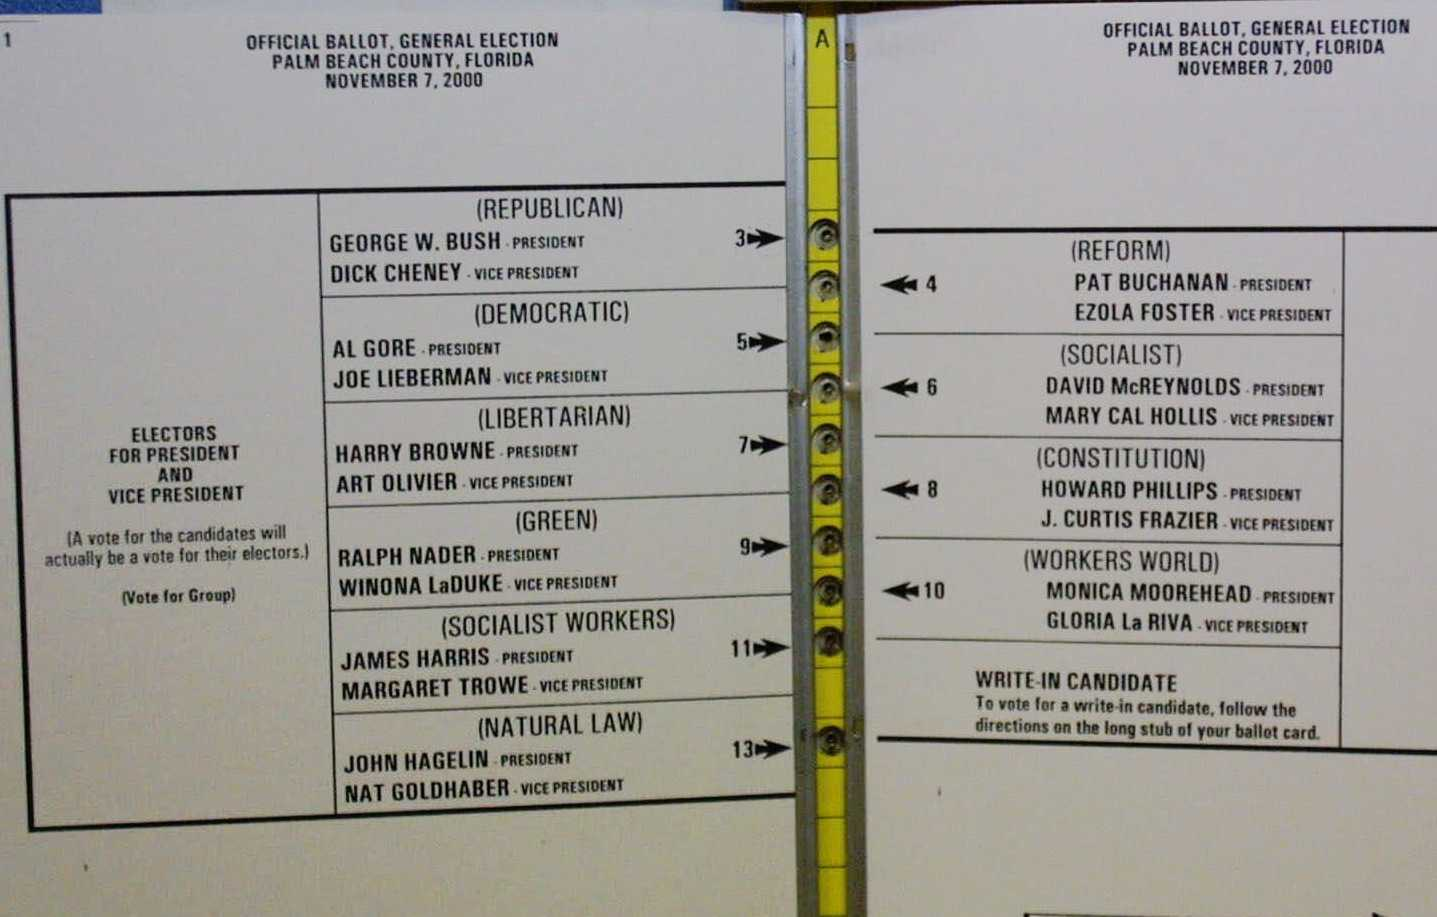
\includegraphics{butterfly.jpg}

In this lab, you will evaluate this. The data file
\texttt{https://raw.githubusercontent.com/dlsun/data-science-book/master/data/florida.csv}
contains county-level information about:

\begin{itemize}
\tightlist
\item
  the number of votes for Gore, Bush, Buchanan (and a few other
  candidates) in the 2000 presidential election
\item
  the number of votes for Clinton (Democrat), Dole (Republican), and
  Perot (Reform) in the 1996 presidential election
\item
  the number of votes for Buchanan in the 1996 primary
\item
  the number of registered Reform voters and the total number of
  registered voters
\end{itemize}

Using this data, evaluate the claim that many voters in Palm Beach
County voted for Buchanan when they intended to vote for Gore.
(\emph{Hint:} You should check whether Palm Beach County fits the
general pattern of the other counties in Florida. Visualizations will
likely be more helpful than summary statistics.) Then, craft a story
that guides the reader through your discoveries. Your story should
contain both figures and explanations.

    \begin{Verbatim}[commandchars=\\\{\}]
{\color{incolor}In [{\color{incolor}11}]:} \PY{k+kn}{import} \PY{n+nn}{pandas} \PY{k}{as} \PY{n+nn}{pd}
         \PY{o}{\PYZpc{}}\PY{k}{matplotlib} inline
         
         \PY{n}{df} \PY{o}{=} \PY{n}{pd}\PY{o}{.}\PY{n}{read\PYZus{}csv}\PY{p}{(}\PY{l+s+s2}{\PYZdq{}}\PY{l+s+s2}{https://raw.githubusercontent.com/dlsun/data\PYZhy{}science\PYZhy{}book/master/data/florida.csv}\PY{l+s+s2}{\PYZdq{}}\PY{p}{)}
         \PY{n}{top\PYZus{}df} \PY{o}{=} \PY{n}{df}\PY{o}{.}\PY{n}{loc}\PY{p}{[}\PY{l+m+mi}{0}\PY{p}{:}\PY{l+m+mi}{48}\PY{p}{,} \PY{p}{:}\PY{p}{]}
         \PY{n}{bottom\PYZus{}df} \PY{o}{=} \PY{n}{df}\PY{o}{.}\PY{n}{loc}\PY{p}{[}\PY{l+m+mi}{49}\PY{p}{:}\PY{p}{,} \PY{p}{:}\PY{p}{]}
         \PY{n}{bottom\PYZus{}df}\PY{o}{.}\PY{n}{loc}\PY{p}{[}\PY{l+m+mi}{49}\PY{p}{,} \PY{l+s+s2}{\PYZdq{}}\PY{l+s+s2}{country}\PY{l+s+s2}{\PYZdq{}}\PY{p}{]} \PY{o}{=} \PY{l+s+s1}{\PYZsq{}}\PY{l+s+s1}{PASCO}\PY{l+s+s1}{\PYZsq{}}
         \PY{n}{pb} \PY{o}{=} \PY{n}{bottom\PYZus{}df}\PY{o}{.}\PY{n}{loc}\PY{p}{[}\PY{l+m+mi}{66}\PY{p}{,} \PY{l+s+s2}{\PYZdq{}}\PY{l+s+s2}{county}\PY{l+s+s2}{\PYZdq{}}\PY{p}{:}\PY{l+s+s2}{\PYZdq{}}\PY{l+s+s2}{buchanan96p}\PY{l+s+s2}{\PYZdq{}}\PY{p}{]}
         \PY{n}{bottom\PYZus{}df}\PY{o}{.}\PY{n}{loc}\PY{p}{[}\PY{p}{:}\PY{p}{,} \PY{l+s+s2}{\PYZdq{}}\PY{l+s+s2}{county}\PY{l+s+s2}{\PYZdq{}}\PY{p}{:}\PY{l+s+s2}{\PYZdq{}}\PY{l+s+s2}{buchanan96p}\PY{l+s+s2}{\PYZdq{}}\PY{p}{]} \PY{o}{=} \PY{p}{(}\PY{n}{bottom\PYZus{}df}
                         \PY{o}{.}\PY{n}{loc}\PY{p}{[}\PY{p}{:}\PY{p}{,} \PY{l+s+s2}{\PYZdq{}}\PY{l+s+s2}{county}\PY{l+s+s2}{\PYZdq{}}\PY{p}{:}\PY{l+s+s2}{\PYZdq{}}\PY{l+s+s2}{buchanan96p}\PY{l+s+s2}{\PYZdq{}}\PY{p}{]}\PY{o}{.}\PY{n}{shift}\PY{p}{(}\PY{l+m+mi}{1}\PY{p}{)}\PY{p}{)}
         \PY{n}{bottom\PYZus{}df}\PY{o}{.}\PY{n}{loc}\PY{p}{[}\PY{l+m+mi}{49}\PY{p}{,} \PY{l+s+s2}{\PYZdq{}}\PY{l+s+s2}{county}\PY{l+s+s2}{\PYZdq{}}\PY{p}{:}\PY{l+s+s2}{\PYZdq{}}\PY{l+s+s2}{buchanan96p}\PY{l+s+s2}{\PYZdq{}}\PY{p}{]} \PY{o}{=} \PY{n}{pb}
         \PY{n}{votes\PYZus{}df} \PY{o}{=} \PY{n}{top\PYZus{}df}\PY{o}{.}\PY{n}{append}\PY{p}{(}\PY{n}{bottom\PYZus{}df}\PY{p}{)}
         \PY{n}{votes\PYZus{}df} \PY{o}{=} \PY{p}{(}\PY{n}{votes\PYZus{}df}\PY{o}{.}\PY{n}{set\PYZus{}index}\PY{p}{(}\PY{l+s+s2}{\PYZdq{}}\PY{l+s+s2}{county}\PY{l+s+s2}{\PYZdq{}}\PY{p}{)}
                     \PY{p}{[}\PY{p}{[}\PY{l+s+s1}{\PYZsq{}}\PY{l+s+s1}{buchanan2000}\PY{l+s+s1}{\PYZsq{}}\PY{p}{,} \PY{l+s+s1}{\PYZsq{}}\PY{l+s+s1}{gore2000}\PY{l+s+s1}{\PYZsq{}}\PY{p}{,} \PY{l+s+s1}{\PYZsq{}}\PY{l+s+s1}{bush2000}\PY{l+s+s1}{\PYZsq{}}\PY{p}{,}
                       \PY{l+s+s1}{\PYZsq{}}\PY{l+s+s1}{nader2000}\PY{l+s+s1}{\PYZsq{}}\PY{p}{,} \PY{l+s+s1}{\PYZsq{}}\PY{l+s+s1}{browne2000}\PY{l+s+s1}{\PYZsq{}}\PY{p}{,} \PY{l+s+s1}{\PYZsq{}}\PY{l+s+s1}{reform.reg}\PY{l+s+s1}{\PYZsq{}}\PY{p}{,} \PY{l+s+s1}{\PYZsq{}}\PY{l+s+s1}{total.reg}\PY{l+s+s1}{\PYZsq{}}\PY{p}{]}\PY{p}{]}\PY{p}{)}
         \PY{k}{for} \PY{n}{col} \PY{o+ow}{in} \PY{n}{votes\PYZus{}df}\PY{p}{:}
             \PY{n}{votes\PYZus{}df}\PY{p}{[}\PY{n}{col}\PY{p}{]} \PY{o}{=} \PY{n}{votes\PYZus{}df}\PY{p}{[}\PY{n}{col}\PY{p}{]}\PY{o}{.}\PY{n}{astype}\PY{p}{(}\PY{n+nb}{str}\PY{p}{)}\PY{o}{.}\PY{n}{str}\PY{o}{.}\PY{n}{replace}\PY{p}{(}\PY{l+s+s2}{\PYZdq{}}\PY{l+s+s2}{,}\PY{l+s+s2}{\PYZdq{}}\PY{p}{,} \PY{l+s+s2}{\PYZdq{}}\PY{l+s+s2}{\PYZdq{}}\PY{p}{)}\PY{o}{.}\PY{n}{astype}\PY{p}{(}\PY{n+nb}{int}\PY{p}{)}
\end{Verbatim}


    \begin{Verbatim}[commandchars=\\\{\}]
/opt/conda/lib/python3.6/site-packages/pandas/core/indexing.py:357: SettingWithCopyWarning: 
A value is trying to be set on a copy of a slice from a DataFrame.
Try using .loc[row\_indexer,col\_indexer] = value instead

See the caveats in the documentation: http://pandas.pydata.org/pandas-docs/stable/indexing.html\#indexing-view-versus-copy
  self.obj[key] = \_infer\_fill\_value(value)
/opt/conda/lib/python3.6/site-packages/pandas/core/indexing.py:537: SettingWithCopyWarning: 
A value is trying to be set on a copy of a slice from a DataFrame.
Try using .loc[row\_indexer,col\_indexer] = value instead

See the caveats in the documentation: http://pandas.pydata.org/pandas-docs/stable/indexing.html\#indexing-view-versus-copy
  self.obj[item] = s

    \end{Verbatim}

    \begin{Verbatim}[commandchars=\\\{\}]
{\color{incolor}In [{\color{incolor}12}]:} \PY{n}{votes\PYZus{}props} \PY{o}{=} \PY{p}{(}\PY{n}{votes\PYZus{}df}\PY{o}{.}\PY{n}{loc}\PY{p}{[}\PY{p}{:}\PY{p}{,} \PY{l+s+s2}{\PYZdq{}}\PY{l+s+s2}{buchanan2000}\PY{l+s+s2}{\PYZdq{}}\PY{p}{:}\PY{l+s+s2}{\PYZdq{}}\PY{l+s+s2}{browne2000}\PY{l+s+s2}{\PYZdq{}}\PY{p}{]}
                        \PY{o}{.}\PY{n}{divide}\PY{p}{(}\PY{n}{votes\PYZus{}df}\PY{o}{.}\PY{n}{loc}\PY{p}{[}\PY{p}{:}\PY{p}{,} \PY{l+s+s2}{\PYZdq{}}\PY{l+s+s2}{buchanan2000}\PY{l+s+s2}{\PYZdq{}}\PY{p}{:}\PY{l+s+s2}{\PYZdq{}}\PY{l+s+s2}{browne2000}\PY{l+s+s2}{\PYZdq{}}\PY{p}{]}
                                \PY{o}{.}\PY{n}{sum}\PY{p}{(}\PY{n}{axis}\PY{o}{=}\PY{l+m+mi}{1}\PY{p}{)}\PY{p}{,} \PY{n}{axis}\PY{o}{=}\PY{l+m+mi}{0}\PY{p}{)}\PY{p}{)}
         \PY{n}{votes\PYZus{}props}\PY{o}{.}\PY{n}{loc}\PY{p}{[}\PY{o}{\PYZti{}}\PY{n}{votes\PYZus{}props}\PY{o}{.}\PY{n}{index}\PY{o}{.}\PY{n}{isin}\PY{p}{(}\PY{p}{[}\PY{l+s+s1}{\PYZsq{}}\PY{l+s+s1}{PALM BEACH}\PY{l+s+s1}{\PYZsq{}}\PY{p}{]}\PY{p}{)}\PY{p}{]}\PY{o}{.}\PY{n}{mean}\PY{p}{(}\PY{p}{)}\PY{o}{.}\PY{n}{plot}\PY{o}{.}\PY{n}{bar}\PY{p}{(}\PY{p}{)}
\end{Verbatim}


\begin{Verbatim}[commandchars=\\\{\}]
{\color{outcolor}Out[{\color{outcolor}12}]:} <matplotlib.axes.\_subplots.AxesSubplot at 0x7f317b31f278>
\end{Verbatim}
            
    \begin{center}
    \adjustimage{max size={0.9\linewidth}{0.9\paperheight}}{output_2_1.png}
    \end{center}
    { \hspace*{\fill} \\}
    
    \begin{Verbatim}[commandchars=\\\{\}]
{\color{incolor}In [{\color{incolor}13}]:} \PY{n}{votes\PYZus{}props}\PY{o}{.}\PY{n}{loc}\PY{p}{[}\PY{l+s+s2}{\PYZdq{}}\PY{l+s+s2}{PALM BEACH}\PY{l+s+s2}{\PYZdq{}}\PY{p}{,} \PY{p}{:}\PY{p}{]}\PY{o}{.}\PY{n}{plot}\PY{o}{.}\PY{n}{bar}\PY{p}{(}\PY{p}{)}
\end{Verbatim}


\begin{Verbatim}[commandchars=\\\{\}]
{\color{outcolor}Out[{\color{outcolor}13}]:} <matplotlib.axes.\_subplots.AxesSubplot at 0x7f317b2adeb8>
\end{Verbatim}
            
    \begin{center}
    \adjustimage{max size={0.9\linewidth}{0.9\paperheight}}{output_3_1.png}
    \end{center}
    { \hspace*{\fill} \\}
    
    At first glance, we can see that Palm Beach county has a larger
proportion of voters that voted for Gore, both in the voter proportions
for Palm Beach and the overall voter proportions as well.

    \begin{Verbatim}[commandchars=\\\{\}]
{\color{incolor}In [{\color{incolor}14}]:} \PY{n}{reform\PYZus{}props} \PY{o}{=} \PY{n}{votes\PYZus{}df}\PY{p}{[}\PY{l+s+s2}{\PYZdq{}}\PY{l+s+s2}{reform.reg}\PY{l+s+s2}{\PYZdq{}}\PY{p}{]} \PY{o}{/} \PY{n}{votes\PYZus{}df}\PY{p}{[}\PY{l+s+s2}{\PYZdq{}}\PY{l+s+s2}{total.reg}\PY{l+s+s2}{\PYZdq{}}\PY{p}{]}
         \PY{n}{reform\PYZus{}props}\PY{o}{.}\PY{n}{loc}\PY{p}{[}\PY{o}{\PYZti{}}\PY{n}{reform\PYZus{}props}\PY{o}{.}\PY{n}{index}\PY{o}{.}\PY{n}{isin}\PY{p}{(}\PY{p}{[}\PY{l+s+s1}{\PYZsq{}}\PY{l+s+s1}{PALM BEACH}\PY{l+s+s1}{\PYZsq{}}\PY{p}{]}\PY{p}{)}\PY{p}{]}\PY{o}{.}\PY{n}{plot}\PY{o}{.}\PY{n}{hist}\PY{p}{(}\PY{p}{)}
\end{Verbatim}


\begin{Verbatim}[commandchars=\\\{\}]
{\color{outcolor}Out[{\color{outcolor}14}]:} <matplotlib.axes.\_subplots.AxesSubplot at 0x7f317b202160>
\end{Verbatim}
            
    \begin{center}
    \adjustimage{max size={0.9\linewidth}{0.9\paperheight}}{output_5_1.png}
    \end{center}
    { \hspace*{\fill} \\}
    
    \begin{Verbatim}[commandchars=\\\{\}]
{\color{incolor}In [{\color{incolor}15}]:} \PY{n}{reform\PYZus{}props}\PY{o}{.}\PY{n}{loc}\PY{p}{[}\PY{l+s+s2}{\PYZdq{}}\PY{l+s+s2}{PALM BEACH}\PY{l+s+s2}{\PYZdq{}}\PY{p}{]}
\end{Verbatim}


\begin{Verbatim}[commandchars=\\\{\}]
{\color{outcolor}Out[{\color{outcolor}15}]:} 0.00051317660889242179
\end{Verbatim}
            
    \begin{Verbatim}[commandchars=\\\{\}]
{\color{incolor}In [{\color{incolor}16}]:} \PY{n}{actual\PYZus{}reform\PYZus{}props} \PY{o}{=} \PY{p}{(}\PY{n}{votes\PYZus{}df}\PY{o}{.}\PY{n}{loc}\PY{p}{[}\PY{p}{:}\PY{p}{,} \PY{l+s+s2}{\PYZdq{}}\PY{l+s+s2}{buchanan2000}\PY{l+s+s2}{\PYZdq{}}\PY{p}{]}
                                \PY{o}{.}\PY{n}{divide}\PY{p}{(}\PY{n}{votes\PYZus{}df}\PY{o}{.}\PY{n}{loc}\PY{p}{[}\PY{p}{:}\PY{p}{,} \PY{l+s+s2}{\PYZdq{}}\PY{l+s+s2}{buchanan2000}\PY{l+s+s2}{\PYZdq{}}\PY{p}{:}\PY{l+s+s2}{\PYZdq{}}\PY{l+s+s2}{browne2000}\PY{l+s+s2}{\PYZdq{}}\PY{p}{]}
                                \PY{o}{.}\PY{n}{sum}\PY{p}{(}\PY{n}{axis}\PY{o}{=}\PY{l+m+mi}{1}\PY{p}{)}\PY{p}{,} \PY{n}{axis}\PY{o}{=}\PY{l+m+mi}{0}\PY{p}{)}\PY{p}{)}
         \PY{n}{actual\PYZus{}reform\PYZus{}props}\PY{o}{.}\PY{n}{plot}\PY{o}{.}\PY{n}{hist}\PY{p}{(}\PY{p}{)}
\end{Verbatim}


\begin{Verbatim}[commandchars=\\\{\}]
{\color{outcolor}Out[{\color{outcolor}16}]:} <matplotlib.axes.\_subplots.AxesSubplot at 0x7f317b183668>
\end{Verbatim}
            
    \begin{center}
    \adjustimage{max size={0.9\linewidth}{0.9\paperheight}}{output_7_1.png}
    \end{center}
    { \hspace*{\fill} \\}
    
    \begin{Verbatim}[commandchars=\\\{\}]
{\color{incolor}In [{\color{incolor}17}]:} \PY{n}{actual\PYZus{}reform\PYZus{}props}\PY{o}{.}\PY{n}{loc}\PY{p}{[}\PY{l+s+s2}{\PYZdq{}}\PY{l+s+s2}{PALM BEACH}\PY{l+s+s2}{\PYZdq{}}\PY{p}{]}
\end{Verbatim}


\begin{Verbatim}[commandchars=\\\{\}]
{\color{outcolor}Out[{\color{outcolor}17}]:} 0.0078956211399636156
\end{Verbatim}
            
    By looking at the difference between the proportion of reform voters
that registered (relative to total registered) and the proportion of
voters that voted reform (relative to total votes), we are able to
create a distribution of those differences. This will help us decide
whether the ballot design had any real effect on the voting numbers.

    \begin{Verbatim}[commandchars=\\\{\}]
{\color{incolor}In [{\color{incolor}18}]:} \PY{n}{reform\PYZus{}props\PYZus{}diff} \PY{o}{=} \PY{n}{actual\PYZus{}reform\PYZus{}props} \PY{o}{\PYZhy{}} \PY{n}{reform\PYZus{}props}
         \PY{n}{reform\PYZus{}props\PYZus{}diff}\PY{o}{.}\PY{n}{loc}\PY{p}{[}\PY{o}{\PYZti{}}\PY{n}{reform\PYZus{}props\PYZus{}diff}\PY{o}{.}\PY{n}{index}\PY{o}{.}\PY{n}{isin}\PY{p}{(}\PY{p}{[}\PY{l+s+s1}{\PYZsq{}}\PY{l+s+s1}{PALM BEACH}\PY{l+s+s1}{\PYZsq{}}\PY{p}{]}\PY{p}{)}\PY{p}{]}\PY{o}{.}\PY{n}{plot}\PY{o}{.}\PY{n}{hist}\PY{p}{(}\PY{p}{)}
\end{Verbatim}


\begin{Verbatim}[commandchars=\\\{\}]
{\color{outcolor}Out[{\color{outcolor}18}]:} <matplotlib.axes.\_subplots.AxesSubplot at 0x7f317b0e2f60>
\end{Verbatim}
            
    \begin{center}
    \adjustimage{max size={0.9\linewidth}{0.9\paperheight}}{output_10_1.png}
    \end{center}
    { \hspace*{\fill} \\}
    
    \begin{Verbatim}[commandchars=\\\{\}]
{\color{incolor}In [{\color{incolor}19}]:} \PY{n}{reform\PYZus{}props\PYZus{}diff}\PY{o}{.}\PY{n}{loc}\PY{p}{[}\PY{l+s+s2}{\PYZdq{}}\PY{l+s+s2}{PALM BEACH}\PY{l+s+s2}{\PYZdq{}}\PY{p}{]}
\end{Verbatim}


\begin{Verbatim}[commandchars=\\\{\}]
{\color{outcolor}Out[{\color{outcolor}19}]:} 0.0073824445310711941
\end{Verbatim}
            
    When compared with the distribution of the reform vote differences
(registered vs actual), the reform turnout for Palm Beach seems
reasonable, and does not seem to have been affected by the ballot. The
Palm Beach difference of approximately (0.0073) is not an outlier in
this distribution, and there exists a number of counties that had around
the same difference. From this, we can conclude that the ballot did not
in fact have any effect of the election.

    \hypertarget{submission-instructions}{%
\section{Submission Instructions}\label{submission-instructions}}

Once you are finished, follow these steps:

\begin{enumerate}
\def\labelenumi{\arabic{enumi}.}
\tightlist
\item
  Restart the kernel and re-run this notebook from beginning to end by
  going to
  \texttt{Kernel\ \textgreater{}\ Restart\ Kernel\ and\ Run\ All\ Cells}.
\item
  If this process stops halfway through, that means there was an error.
  Correct the error and repeat Step 1 until the notebook runs from
  beginning to end.
\item
  Double check that there is a number next to each code cell and that
  these numbers are in order.
\end{enumerate}

Then, submit your lab as follows:

\begin{enumerate}
\def\labelenumi{\arabic{enumi}.}
\tightlist
\item
  Go to
  \texttt{File\ \textgreater{}\ Export\ Notebook\ As\ \textgreater{}\ PDF}.
\item
  Double check that the entire notebook, from beginning to end, is in
  this PDF file. (If the notebook is cut off, try first exporting the
  notebook to HTML and printing to PDF.)
\item
  Upload the PDF
  \href{https://polylearn.calpoly.edu/AY_2018-2019/mod/assign/view.php?id=313949}{to
  PolyLearn}.
\end{enumerate}


    % Add a bibliography block to the postdoc
    
    
    
    \end{document}
